\documentclass[12pt]{article}
\usepackage{lmodern, amssymb,amsmath, graphicx, hyperref}
% === bibliography package ===
\usepackage{natbib}
% \usepackage[colorinlistoftodos, prependcaption]{todonotes} % to use \todo 
\usepackage[margin=1in]{geometry}
\usepackage{csquotes}
\usepackage{lscape}
\usepackage{setspace}
\hypersetup{
    colorlinks=true,
    linkcolor=blue,
    filecolor=magenta,      
    urlcolor=cyan,
    citecolor = black
}
\newenvironment{tight_itemize}{
\begin{itemize}
  \setlength{\itemsep}{0pt}
  \setlength{\parskip}{0pt}
 }{\end{itemize}}
\urlstyle{same}  % don't use monospace font for urls

  \title{Unequal Representation: Evidence from a Census of US Federal Agencies}
    \author{Devin Judge-Lord\thanks{Ph.D. Candidate, University of Wisconsin-Madison}\and Justin Grimmer\thanks{Professor, Stanford University and Senior Fellow, Hoover Institution} \and Eleanor Neff Powell\thanks{Booth Fowler Associate Professor, University of Wisconsin-Madison}}
    \date{\today}
    
\graphicspath{{gh-pages/Figs/}}

\usepackage{booktabs} % To thicken table lines

\bibliographystyle{apsr}


\begin{document}

\maketitle
% \tableofcontents

% \bigskip
% \href{https://judgelord.github.io/correspondence/gh-pages/summary.html}{Project Summary} | 
% \href{https://docs.google.com/document/d/1fJxjXjAyRL9vX-16fSsH29anXZc-W74GMf_7BSgWkws/edit}{Codebook} |
% \bigskip


%%relate this to quality of representation. 

\begin{abstract}
\noindent 
Do members of Congress use increased power and experience to provide greater constituency service or to affect broad public policies? To examine how increased power and experience affect legislators' provision of service, we assemble a massive new database of over 470,000 Congressional requests to agencies between 2007 and 2018 obtained through over \input{../tables/foia_requests} FOIA requests, a near census of federal departments, agencies, and sub-agencies. Using this data set, we demonstrate that experience and power results in more overall constituency service for district residents, even though powerful legislators allocate a larger share of their efforts towards broad public policy goals. After their election, new legislators incur start-up costs and provide less service, but this difference erodes after two years. When legislators acquire more power in Washington---particularly committee chairmanships---they increase constituency service and their oversight of agencies. In a series of robustness checks, we show that our findings are not the result of constituent demand, nor is it merely a result of voters more easily recognizing more experienced legislators. Rather than experienced and powerful legislators focusing their efforts in Washington and away from their district, we demonstrate that legislators use increased resources to provide more services for constituents. 
\end{abstract}



%\input{/users/justingrimmer/correspondence/data/foia_requests}

%\input{/users/justingrimmer/correspondence/data/n}

\newpage
\doublespacing
\section{Introduction}

One of the oldest traditions of legislative representation in American politics is that of constituency service---the ways in which legislators help to channel and articulate individual constituent's requests to the government.  Constituency service is when Members of Congress ``provid[e] help to individuals, groups, and localities in coping with the federal government" \citep{Fenno1978}.\footnote{This tradition of constituency service can be traced back to the first congresses when constituents sought assistance with Revolutionary War pensions \citep{Eckman2017} and continues today as constituents seek assistance with a wide range of topics from Social Security, Disability, and Veterans Benefits to Citizenship Applications to complaints about pollution and employment discrimination.} Advocating on behalf of their constituents to federal agencies is an important facet of modern legislators' jobs, and its growth has been used to explain the presence of the incumbency advantage \citep{King1991}. Yet despite the centrality of constituency service in theories of congressional representation, constituency service remains one of the most opaque and least understood congressional activities.\footnote{Modern constituency service encompasses much more than the oft-cited examples of helping constituents with federal benefits. Members also serve constituents by seeking to help intercede on their behalf with a host of lesser-known federal agencies as well as advocating on behalf of state or local governments or nonprofits who apply for federal grants, permits, or disaster recovery funds.}  Indeed, we are not the first to observe the relative lack of empirical attention to constituency service in the literature.  Over thirty years ago \citet*{CainFerejohnFiorina1987} began their seminal book \emph{The Personal Vote: Constituency Service and Electoral Independence} with that same observation, and much of what we know empirically today about constituency service comes from their surveys of legislators, legislative staff, and constituents. The disproportionate academic focus on representative's legislative activities, has left unanswered long-standing questions about how legislators balance the pursuit of legislative goals in Washington with the provision of constituency service. 
% \todo{include other examples of constituency service} \citep{Eckman2017} 
%Everythign a legislator does is legislator advocacy
% The full group---all legislators do for categories individuals, groups, and businesses---that is constituent advocacy.  Then categories 4-5 are policy advocacy. 
%The final level---individual level help.  Category 1 only.  

%CAPACITY IS BUDGET AND COMPETENCE. AND COMPETENCE CAN BE LEARNED.  
%EMBEDDEDNESS.  IT IS A DOUBLE EDGE SWORD.  BUILDING NETWORKS AND RELATIONSHIP.  BUILDING A SYSTEM.  

%%PROVIDE MORE EFFICIENTLY, OR FOCUS ON WORK IN WASHINGTON 

We tackle these classic empirical questions about constituency service with a new approach---by looking at when legislators contact government agencies on behalf of their constituents using a novel dataset of congressional contact with all federal agencies.  Recent work using data on congressional correspondence has yielded important findings regarding the policy strategies of cross-pressured legislators \citep{Ritchie2017}, distributive politics \citep{MillsKalafHuges2015}, descriptive representation \citep{LowandeRitchieLauterbach2018}, and the role of ideology in congressional oversight \citep{Lowande2018JOP}.  

We build on their work and formal models of legislative accountability to test competing expectations about how legislators' experience and power in Washington will affect the amount of constituency service they provide constituents back home \citep{AshworthBuenodeMesquita2006}.  On the one hand, we might expect increased power in Washington and experience in the institution will increase the levels of service, because experience and power increases legislators' capacity to provide service.  When legislators are newly elected they pay start up costs as they hire staff and organize their office, causing lower capacity to deliver service.  And as legislators move to more prestigious committees or become committee chairpersons, they gain access to additional committee resources, enabling legislators to allocate their office resources to provide service to the district.  

On the other hand, we might expect that as legislators spend more time in Washington and gain prestige they become less attentive to the district and their constituents and therefore decrease levels of service provided to constituents, even as their capacity increases. This is articulated in theories of representation with a perceived trade-off between experienced legislators who wield institutional power within Washington and more recently elected legislators who are attentive to the district.  As legislators acquire power in the institution, it is often asserted that they catch ``Potomac fever'' and devote less attention to constituents back in the district \citep{Fenno1978}.  A similar argument is made in the popular press \citep{Edwards2005} and evoked in rallying cries to ``drain the swamp'' of politicians accused paying too much attention to Washington policy elite and not enough attention to their constituents back home \citep{Rosenblatt2016}.  It seems intuitive that as they spend more time in Washington and assume more important roles in Congress, legislators would have less time for individual constituents and prioritize constituency service at lower rates than their constituents desire.  As attention drifts, we might also imagine that legislators allocate more of their resources towards their policy work.  This might be particularly true as representatives occupy increasingly powerful positions in the institution---such as committee chairs or obtain seats on prestigious committees. While committee chairs have additional staff to handle legislative affairs, supervising these staff may direct a chairs' attention to policy work. 



%Drawing on formal models of accountability (for example, ), we might expect that if constituency service enables elected officials to demonstrate competence to their constituents, then increased power and resources in Washington will result in increased levels of service to constituents.  This increase in service occurs as legislators either siphon off some of their increased resources or use the increased resources that come with better committee assignments fungibly,  allowing them to shift more effort to constituency service to satisfy the primary goal of reelection.  Similarly, it could be that newly elected members of Congress incur start-up costs when they enter office.  If start up costs are present, then incumbent legislators have an advantage, because their replacements---even if they will be more competent eventually---will necessarily provide less constituency service at the outset, but the level of service will rise as legislators hire staff and they establish a system for handling constituency caseload.  


%As several formal models demonstrate constituency service, on its own, is insufficient to explain an incumbency advantage.  This is because if all elected legislators provide equal amounts of service, then constituents are indifferent between the service that one incumbent would provide to a replacement.  Rather, for constituency service to provide an advantage, it must be that constituents have evidence from that service that the current incumbent provides them with some advantage over a potential replacement.  .  Or, it could be that constituency service provides evidence of an elected officials' competence.  If true, then increases in a legislators' resources as they gain expertise leads to the expectation that they provide more constituency service (Ashworth and Bueno de Mesquita CITE).  


%%BE CLEAR ABOUT CAPACITY AND HOW WE"RE GOING TO DECOMPOSE THAT CAPACITY
%%CLARIFY CONSTITUENCY FROM POLICY WORK.  USE DIFFERENT WORDS DISTRICT ADVOCACY 
%%CONSTITUENT SERVICE 


To test how legislators alter constituency service with changes in power in Congress and experience in Washington, we built a massive new dataset of constituency service requests to understand how legislators provision of service changes as they gain expertise and experience in the institution.  To demonstrate how institutional power affects district attention, we utilize a new data set of 470,484 correspondences between members of Congress and constituents we compiled through hundreds of Freedom of Information Act requests. Using this new data set, we show that most contact with federal agencies is made on behalf of constituents.  Using a manual hand-coding of the content of service requests, we show that nearly 90\% of requests are made on behalf of constituents and only 10\% are focused on policy related federal oversight.  In general, the legislators who engage the bureaucracy do so broadly, across many agencies and advocate both for general policy and for individual constituents.   

%we also establish some important stylized facts about when and how elected officials contact federal agencies. We show that letter writing is not evenly distributed. Some members simply use this tactic more than others, even within strata of institutional power. Legislators' district characteristics also helps explain their use of constituency service: senators from larger states make more requests.  And legislators whose districts are composed of a larger proportion of veterans make more requests to the Veterans' Administration, while those represent districts with a larger proportion of older residents make more requests to the Social Security Administration.  We also 

Using our new data set of constituency service requests, we show that as legislators spend more time in Congress they acquire expertise and access to resources that increase their provision of constituency service, rather than directing attention away from the district.  Using a within-legislator-agency pair difference-in-differences design, we show that more power causes legislators to provide more constituency service.  Using a similar difference-in-differences design, we also show that newly elected legislators make fewer constituency service requests and that electing a new legislator causes a large drop in constituency service requests from a district's representative.  We show that this difference is not due to selection in the sophomore election: we find a near identical effect when we restrict our analysis to representatives who last until their third year in office.  Further, we show that legislators continue focusing on constituency service when contacting federal agencies as they acquire more power and experience in Washington.  

Through a series of robustness checks and additional analyses, we show that the effects we identify are not the result of constituents strategically changing their demands for help, rather than reflecting changes in legislator effort.  We show that there is little evidence that individuals shift responses to more established offices when a new representative is elected.  When House members lose an election, there is no corresponding increase in constituency service requests from the state's Senate delegation.  Further, we show that more prestigious committee assignments do not increase representative's name recognition and that the increase in name recognition that comes from a longer tenure in Washington does not align with the changes in constituency service over a legislator's tenure.  Finally, our research designs limit the influence of constituent demand that might be present, by ensuring that we make within district comparisons.  

Our results provide important new insights into how elected officials allocate their effort over their legislative career.  We demonstrate that incumbents' acquisition of experience and power in Washington not only enables them to transmit their constituents' views more effectively through policy representation and influence.  It also enables these legislators to increase the amount of constituency service provided to the district.  This suggests that constituents with experienced legislators are able to benefit from that experience and increased prestige---demonstrating that there is no tradeoff between increased policy demand in the institution and particularlistic goods in the district.  Our results also help to explain how constituency service can contribute to the incumbency advantage: when constituents choose between legislators, the choice to replace an incumbent legislator comes at the cost of less constituency service. It also shows that popular concerns of legislators who have spent too much time in Washington and have lost touch with the district are misplaced.  Rather, it is the legislators who have acquired experience and power in Washington who are best placed to deliver service for their constituents.    

This paper proceeds as follows.  Section \ref{s:theory} explains divergent predictions about how legislators' effort will be affected by institutional position and tenure in Congress.  In Section \ref{s:data} we explain our data collection process and provide basic summary statistics.  Sections \ref{s:prestige} and \ref{s:tenure} show that better committee assignments and increased tenure cause more constituency service.  And Section \ref{s:demand} provides robustness checks for our results and explores alternative explanations.  We conclude in Section \ref{s:conclude}


\section{How Does Experience and Power Affect Constituency Service?} \label{s:theory}

A tension in representation is how legislators balance their work on national level policy---such as passing legislation---and delivering particularistic goods to their constituents and district---such as providing constituent service \citep{AshworthBuenodeMesquita2006}.  Legislators contact the bureaucracy to build support with constituents, because federal agencies have strong incentives to be responsive to elected officials. In fulfilling statutory missions, agencies must prioritize resources and use broad discretion, not only in processing visa, permit, and grant applications but in regulating private entities' compliance with, for example, environmental, health, and labor laws. For a vast range of demands involving public or private actors, a federal agency will often be able to help if it prioritizes that demand over others. 

Legislators are in a position to influence agency decisions. As public servants, agency staff may assign special importance to the demands of elected officials.  For example, many agencies tag congressional correspondence as ``VIP" and agency protocols often require faster response deadlines and higher signature levels. Agencies also have strategic reasons to meet congressional demands. Ad hoc review of a social security disbursement, visa application, or pipeline permit may be inefficient and diverge from protocol but nevertheless, a small price to pay if it could help the agency gain a small advantage in securing desired authorizations and budgets.  Bureaucrats have incentives to build relationships and reputations that enhance their standing among members of Congress and those who have their ear, and they actively do so \citep{Carpenter2001}.  In short, complying with legislator request may help agencies achieve their own goals.  If an agency aims to grow its coalition of political supporters, we would expect them to frequently accommodate congressional requests.

Legislators' experience in Washington and their acquisition of power in the institution, are likely to affect how they strike the balance between delivering service to constituents and working on broader legislation.  But comparative statistics from formal models of accountability have divergent predictions of how increased power and experience will affect legislators' attentiveness to the district.  Building on multi-task models of representation \cite{AshworthBuenodeMesquita2006, gordon2009advantages}, we explain why we might expect increased experience and power to either increase or decrease the levels of constituency service legislators provide.  



%But there are competing theoretical expectations of how increased experience and power will affect how much constituency service legislators provide constituents and the kind of service they provide.  On the one hand, formal models of constituency service predict that increased experience and power will cause legislators to bolster the amount of constituency service provided.  Related to these models is the expectation that a new legislator will face significant start up costs as they hire new staff and establish the procedures that will effectively handle the constituency service case load.  After these costs are incurred, constituency service would increase.  On the other hand, concerns about legislators becoming fixated on careers in Washington lead to an expectation that power in Washington comes at the expense of constituencies, as legislators allocate more of their resources and efforts to influencing national level legislation.   In this section, we explicate the logic of these distinct theoretical expectations in this section and explain why it is unclear how legislators with greater experience or prestige will alter their constituency service to constituents.  

\subsection{Why Experience and Power Could Increase Legislators' Constituency Service Effort}

%%THERE IS AN ABSOLUTE AND RELATIVE ARTICULATION OF THE HYPOTHESIS
%%ABSOLUTE IS THAT THE EFFORT WILL GO DOWN COMPLETELY AND INDIVIDUALS WILL LOSE THEIR ATTENTIVESS.  THE RELATIVE IMPLICATION IS THAT A SMALLER SHARE OF THE LEGISLATORS OVERALL EFFORT. THE THEORY IS LARGELY SILENT.  

As elected officials garner more experience in Congress, one prediction from formal models of accountability is that legislators will provide more constituency service, because their capacity to do so increases.  An influential set of formal theory papers argue that constituents are fundamentally engaged in a screening task: attempting to identify elected officials who are competent and able to effectively deliver representation to the district \citep{AshworthBuenodeMesquita2006, gordon2009advantages}.  Under this model of representation, constituency service helps reelection minded legislators increase their chance of reelection if legislators are able to exceed constituent's expectations of the kinds of service that legislators will provide constituents.  

Critically, constituents' demands for service and for legislators to demonstrate their competence do not go away, even as legislators acquire power in the institution.  For example, after Richard Lugar (R-IN) lost a primary election to Richard Mourdock (R-IN) in 2012, analysts argued that ``At its heart, Lugar's defeat was attributable to the fact that he broke the political golden rule: Never lose touch with the people who elected you".\footnote{\url{https://www.washingtonpost.com/blogs/the-fix/post/why-dick-lugar-lost/2012/05/09/gIQAj9cfCU_blog.html}}  More generally, we might expect that even if constituents are supportive of the power their representative has over policy, they still expect that those elected officials will be attentive to the district and to demonstrate their competence with constituency service.  This would induce elected officials to continue to focus on providing services to the district, in order to sustain their chance of reelection.       %https://www.washingtonpost.com/blogs/the-fix/post/why-dick-lugar-lost/2012/05/09/gIQAj9cfCU_blog.html?noredirect=on

%%Paragraph here on how prestige comes with more resources?  

All else equal, then, these models predict that as a legislator's resources increase, they will increase their levels of constituency service \cite[Proposition 1]{AshworthBuenodeMesquita2006}.  There are two mechanisms that will be observationally equivalent for our results: increased resources and an increased likelihood of success when making a request.  First, as legislators acquire more prestige in Washington then they usually acquire more resources.  For example, becoming chair of a Congressional committee provides legislators with better access to committee staff and a larger budget.  Even if these resources are earmarked for policy work, they can increase the resources legislators have available for constituency service. This is because legislators with more access to committee resources can use those resources for policy work, while then focusing the office resources on delivering constituency service.  Second, as legislators become more powerful then agencies have a great incentive to be responsive.  More powerful legislators can more easily alter an agency's budget or create additional work through Congressional hearings.  As a result, agencies often prioritize the service requests from the most powerful members of Congress.  The increased likelihood of a response provides legislators with the opportunity to demonstrate their effectiveness to their constituents. This increases the marginal return on making service requests, providing more prestigious legislators with more incentive to make those requests.   

%One mechanism is that legislators could redirect some of the increased resources that come with increased prestige to the provision of constituency service.  A second different mechanism would occur if legislators move policy focused efforts towards the newly acquired institutional resources.  If the staff resources are fungible, then this would enable legislators to utilize their prior office resources for providing constituency service.  The result of either mechanism is that the additional resources that come with increased prestige lead to more constituency service to constituents.  

Using a similar logic, we also expect that new legislators will face ``start up" costs that will result in them making fewer constituency service requests to agencies.  When a new legislator is elected to office, they face a substantial administrative burden.  Not only does that legislator have to hire new staff and open district offices.  The legislator also needs to establish protocols, priorities, and procedures in their office for handling constituency service requests.  They also lack many of the ``standard" responses that more established offices will use to handle particular kinds of letters.  In terms of formal models, the initial lack of office organization essentially decreases the resources the legislator has available \citep{AshworthBuenodeMesquita2006}.  As legislators build an office and establish protocols, these start up costs should subside and legislators are able to make full use of the resources available to their office.  And as a result, we would expect new legislators to make fewer constituency service requests, but only as they establish their constituency service operation within the office.    

%Building off of this similar logic leads to an expectation that newly elected legislators will provide lower levels of constituency service than returning incumbents, but that this difference will erase after an office establishes their constituency service operation.  If elected officials face an unchanging demand from constituents to provide services to navigate the government, then we would not expect legislators to decrease the service provided to constituents over time.  Yet, newly elected officials are quite likely to pay significant start up costs when organizing their office after the election. Not only are the newly elected officials forced to hire a completely new set of staffers, t.   

\subsection{Why Experience and Power Could Decrease Legislators' Constituency Service Efforts}

An alternative theoretical expectation is that as legislators spend more time in Washington, they become detached from their district.  This concern is present in the political science literature on Congressional careers. Richard Fenno documents that some members of Congress catch ``Potomac fever".  While newly elected legislators may remain primarily focused on re-election, more senior legislators may prioritize other goals. As legislators acquire power in Congress, it is often asserted that they ``go Washington'' and devote less attention to constituents back in the district \citep{Fenno1978}.  It seems intuitive that as they spend more time in Washington and attain more influential institutional roles in Congress, legislators might focus on other priorities resulting in less attention paid to constituents.   While Mayhew emphasizes re-election as the primary goal that motivates legislators, \citet{Fenno1973} identifies five goals: re-election, power in the House, good public policy, a career beyond the House, and private gain.  As Fenno describes in \textit{Congressmen In Committees}, different institutional positions (congressional committees) can be more or less useful to accomplish these goals.  Some committees may be more useful for achieving re-election, because they position you to be of service to your constituents, other committees may not be valued by constituents, but could be used to influence foreign policy, or still other committees might help a member achieve wealth or jobs in the future via lobbying positions or corporate board seats down the road.     

A parallel argument about legislator behavior emerges in public advocacy for reforms in Washington, in particular with activists who advocate for term limits.  These activists argue that elected officials who are repeatedly re-elected to Congress become detached from their district.  For example, Ted Cruz (R-TX) argued in favor of term limits in a Senate hearing, stating that the politicians at the time of founding traveled to Washington and then planned to return to their district.  In its place, Cruz argued that ``Today, members of Congress aren't doing that. Instead, far too many of our politicians come to Washington to stay".  Alexandria Ocasio-Cortez made a similar indictment against Joe Crowley in her successful primary challenge.  She would regularly remind audiences that Crowley had ``been there for 20 years" and then ask, ``What has this power been used for? It's not being used for us."  %https://www.termlimits.com/senator-ted-cruz-hearing/ https://www.thenation.com/article/alexandria-ocasio-cortez-fights-power/

All else equal, formal models of representation predict that as legislators prioritize their work in Washington,  they will provide lower levels of constituency service to their district and the ratio of constituency service to public good provision will decrease.  For example, in the model in \cite{AshworthBuenodeMesquita2006} this would occur as legislators place give lower priority to constituency service than desired by constituents (or than legislators have provided previously).  If members shift their focus from the district to a career in Washington, we should expect that their attention to constituent issues will also decrease.  This would occur as more experienced legislators allocate staff to address broad legislation in Washington, or as legislators who acquire more power focus their efforts on law making, rather than delivering goods to the district.   


\paragraph{Relative vs Absolute Shifts} Of course, legislators experience career shifts that both increase their resources and affect the priority they place on constituency service.  The effect of these off-setting shifts on levels of constituency service will depend on the relative size of legislators' resource increase (or the increased responsiveness of the agency bureaucrats) and the amount they prioritize their constituency service work. And as a result it is possible that even though legislators will prioritize constituency service less after they gain power, their increased resources (or increased agency responsiveness) more than compensates for this shift in focus.  

If this occurs, we will expect that as legislators gain experience they will increase the amount of constituency service provided, but they will increase their policy-work.  So even though we would see increases in the levels of service, we would expect the ratio of constituent service to non-constituency service legislative work to decrease.  


\subsection{Alternative Explanation for Changes in Constituency Service: Constituent Demand}

Our key theoretical puzzle is to understand how legislators' effort for constituents changes as they gain power and experience in Washington. But usually legislators depend on constituents to first ask for help navigating the federal bureaucracy.  An alternative explanation for why legislators' rates of constituency service provision vary is that they receive differing numbers of requests from constituents.  While this would still be interesting substantively, a constituent demand explanation for the provision of constituency service would suggest that varying levels of service provision do not inform debates about how legislator effort changes over their time in Washington. 

Of course, we should expect that constituent demand will inform what agencies legislators contact.  For example, some districts will be comprised of groups---such as veterans or social security recipients---who will request particular kinds of constituency service from their representative.  Our designs will attempt to limit the influence of this kind of constituent demand by examining how an individual legislator's rates of contact changes within particular agencies.  By looking at the same member representing the same constituents in the same district within a particular agency we should be limit the extent to which differing constituent populations could interfere with our results. 

A more challenging form of constituent demand explanation would be if constituents redirect their requests towards legislators who they expect to be more powerful.  For example, we might hypothesize that as legislators acquire more power in Washington they are more easily recognized by their constituents and therefore more likely to receive requests for help from constituents.  Constituents might also expect that more powerful legislators could more effectively provide constituency service and as a result direct service requests towards those legislators.  Similarly, it could be the case that as legislators gain more experience in Washington they are more easily recognized by constituents and, as a result, more likely to receive constituency service requests. 

To address these sorts of constituency demand concerns centered on constituents directing their requests toward legislators they know better, in Section \ref{s:demand} we focus on a series of robustness checks to rule out alternative constituency demand explanations. In particular we examine the limited effects of prestige and tenure on constituent's name recognition of legislators and assess whether there is evidence of constituents redirecting their queries away from new legislators toward incumbent legislators from the same state. 

While we will assess implications of constituency demand for our results in our robustness check section, we also note that constituency demand could also be closely related to legislator effort. Elected officials can encourage requests for help navigating the federal bureaucracy through workshops, newsletters to constituents, and even stories in local papers.  If the prevalence of these stories reflects legislators focus on the district, then increases in requests from constituents could reflect the effort of elected officials.  

\section{A Comprehensive Data Set of Constituent Service Requests} \label{s:data}
To test how experience and power affect the provision of constituent service, we utilize an original collection of constituent service requests, collected from \input{../tables/foia_requests} FOIA requests we made to federal agencies and sub-agencies.  Through our collection process, we have received data on \input{../tables/n} instances of members of Congress contacting federal agencies.  We focus on requests made from 2007-2017, resulting in a data set of 470,484 contacts from members of Congress with federal agencies.   

\subsection{Hundreds of FOIA Requests to Assess Congressional Communication with the Bureaucracy}
To assess when and how members of Congress communicate with the bureaucracy, we conducted---to the best of our ability---a census of federal agencies and sub-agency communication.  Specifically, we identified all departments, agencies, and sub-agencies and submitted requests for all communication with members of Congress from 2007-2018.  To date, we have received records from every department other than the Department of State.  While the specific the length of records to our response might vary over time, our most stringent specifications will include legislator-by-agency fixed effects, which ensures that our comparisons are made within agency.  This limits the opportunity for left-censoring to affect our conclusions.  %%%% Devin can you add a footnote to the Department of State reference that indicates how long the backlog at state is?  Would be nice to explain why we're missing it.  

\paragraph{Variation in Responses to Identical FOIA Request} Responses to our FOIA requests varied significantly. Most agencies offered logs of congressional correspondence, which record a date, sender, and summary of each contact. Logs generally include any written requests, as well as many phone and email records. For example, Between May 2015 and December 2017, the Department of Justice Office of Administrative Law Judges received 132 emails, 109 telephone calls, and only 54 letters. Between 2007 and 2017, the Postal Regulatory Commission received 100 emails, 30 faxes, 173 letters, 118 calls. In this paper, we use ``contacts'' and ``letters'' interchangeably to refer to all modes of correspondence. Small agencies or regional offices had staff search their email history or provided hand-written records that we had transcribed.  Department Secretary offices generally queried a correspondence tracking database designed to track all correspondence, but our FOIA requests to sub-departmental components almost always recovered additional records of communication that was not in central databases. As one central office FOIA officer put it ``Legislative Affairs is supposed to be the front door for the department, but if somebody knows somebody, well...'' (personal communication, Feb. 21, 2018). Because of such idiosyncratic relationships, capturing patterns of correspondence that ``go around'' a Department Secretary's office is key to avoiding erroneous inferences about legislator behavior. For example, when chairs of the Homeland Security committee wrote about immigration enforcement issues, they almost always contacted the Department of Homeland Security (DHS) office of the Executive Secretary, but, at the same time, the Immigration Customs Enforcement (ICE) component of DHS directly received thousands of contacts from a different set of legislators. Our census approach ensures that we capture the totality of legislators' behavior. 

Upon receiving the records, we extracted names matching variations of legislators' names and then merge in data about their position in Washington, district, and career.  In Appendix \ref{a:codebook} we provide our procedure for converting the raw files from federal agencies into the a data set appropriate for analysis.  For approximately half of our contacts we also use the brief description included in the data set to classify the reason for contacting federal agencies.   Our coding process began with the authors coding a representative sample of records. We then trained undergraduate and graduate RAs. The first several thousand letters or log entries were double coded. For example, of over 10,000 log entries for the Environmental Protection Agency, the first 2,500 were double-coded.  Our overall inter-coder agreement was 0.78, which rose to 0.9 when we subsetted our analysis to coding decisions where the coders had a great deal of certainty.  Throughout the hand-coding process, we also developed subagency-specific coding rules where certain regular expressions indicated certain types of correspondence. For example, where "rulemaking" consistently indicated that a legislator's request involved an agency rule, all cases yet uncoded by hand for that agency are assigned to be type "Policy-Rulemaking" for the present analysis.    

We have classified a sample of correspondences, 194,251, into five categories: ``Individual Constituent Service'' (i.e. casework or advocacy on behalf of a group such as employees of a company), ``Nonprofit or Local Government Constituent Service'' (e.g. help with a grant application), ``Corporate Constituent Service'' (e.g. help with a contract), ``Corporate Policy'' (e.g. policy explicitly aimed to benefit a specific industry), and ``Policy'' (general policy work related to legislation, budgets, or rulemaking).  We define constituents broadly such that they need not be in a member's district. For example, Representative Tauscher of Wisconsin wrote to the Defense Commissary Agency on behalf of the Jelly Belly Candy Co., based in California. Jelly Belly was then ``given a chance to resolve issues" with their contract. This was coded as ``Corporate Constituent Service'' and included in our broader measure of constituent service.  We also consider constituent service as broader than casework. For example, Senator Rubio asking the IRS for special treatment for residents of hurricane-affected parts of Florida was coded as ``Individual Constituent Service.'' We note these ``hard cases'' to illustrate the boundaries of our coding scheme. Most contacts were more easily parsed into either individual casework or policy work related to hearings, regulations, and legislation.


\subsection{Who Contacts the Bureaucracy?}
Before testing how legislators' efforts to provide constituency service change as they acquire prestige and experience, we first use our extensive data set of constituency contacts, to establish novel facts about how legislators contact federal agencies and why they contact those agencies.  Overall, we demonstrate that there is considerable variability in the rates legislators contact federal agencies, but we find surprising consistency in the purpose of the communication: when legislators contact federal agencies, they are primarily focused on providing constituency service, with only a small fraction focused on policy.  And we show that legislators are responsive to demographic characteristics of their constituency, but there is still considerable variability in contact rates within quite similar districts.   

\subsubsection{Rates of Contact with Federal Agencies}
Legislators vary a great deal in how much they contact federal agencies.  Figure \ref{f:contact1} shows the average number of contact rates per year for House members (left-hand panel) and senators (right-hand panel).  In the Senate Robert Byrd (D-WV) had an average rate of constituency service provision of 433 constituent service contacts per year.  Other senators---such as Charles Schumer (D-NY) and John McCain (R-AZ)---have similarly high rates of contacted federal agencies.  But other senators contact at a much lower rate.  For example, John Kennedy (R-LA) made 5 constituency service requests during his first year in the Senate in 2017.  On average, senators in our data set contact federal agencies 86 times per year.    
 
\begin{figure}
\centering
\caption{Variation in Across Legislator Contact Rates} \label{f:contact1} 
\begin{minipage}{\textwidth}
\scalebox{0.4}{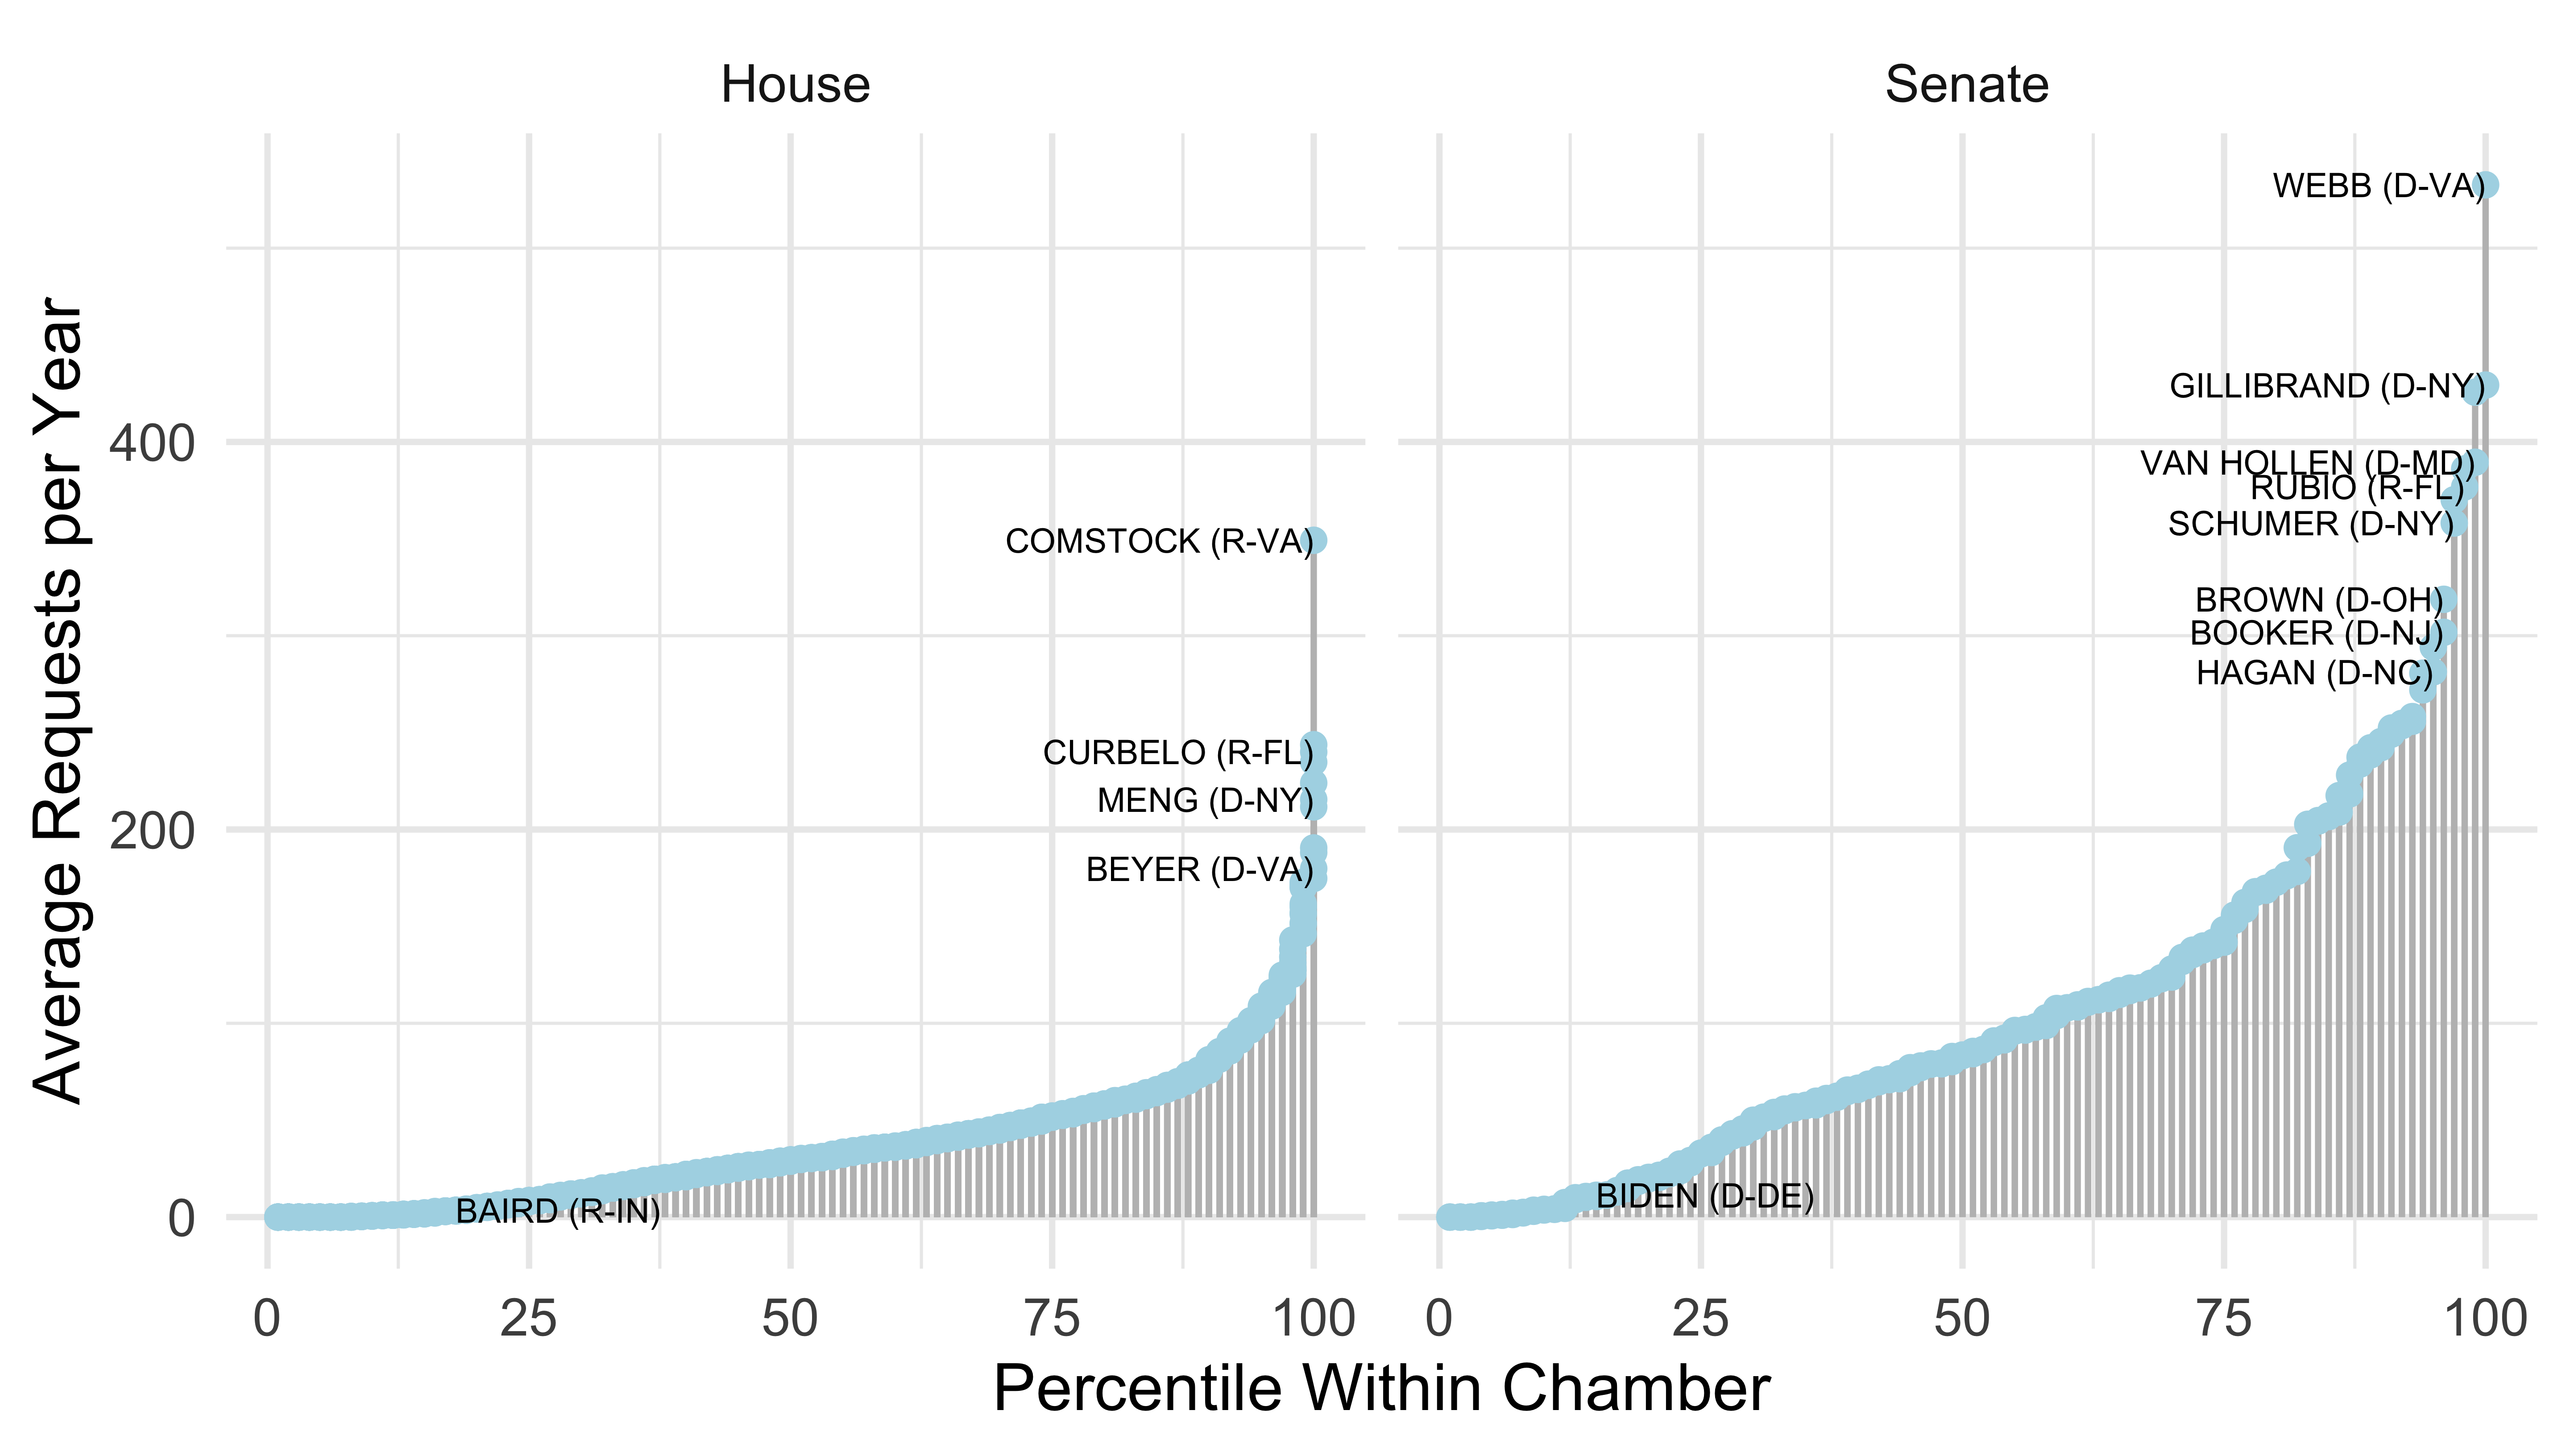
\includegraphics{../figs/percentiles-1}}
\footnotetext{This figure presents the average number of contacts with federal agencies per year for House members (left-hand panel) and senators (right-hand panel), where the legislators' counts are sorted by their per year percentile rank.  This reveals that senators and House members regularly contact federal agencies, but there is considerable variation in the rates of contact across legislators.}
\end{minipage}
\end{figure}

We see similar variation in the House, but with overall lower rates of contacting federal agencies---reflecting the demographic and resource differences across the two institutions.  Frank Wolf (R-VA) had the highest rate of contact with federal agencies, averaging 306 contacts per year. Like the Senate, other legislators contacted at a much lower rate.  Overall, House members averaged 29.4 contacts with federal agencies per year.  But like the Senate we considerable variability in the rates of contact across House members.   

\subsubsection{Legislator's Contact with Federal Agencies are Focused on Constituency Service}
Overall, when legislators contact federal agencies in our sample they are helping constituents navigate the federal bureaucracy.  To reach the conclusion that contacts with federal agencies are constituency service focused, we use our hand-coded sample of legislative contacts and examine the distribution of reasons why legislators contact federal agencies.  Figure \ref{f:type2}, uses our most granular coding scheme and the proportion of contacts that fall within each category.  The left-hand bar shows that 76\% of all contacts with federal agencies are made on behalf of individual constituents.  A smaller percentage, 6\%,  is focused on constituent service requests for corporations in the district and 8\% of requests are made on behalf of non-profits and local governments.  We do find that legislators contact federal agencies to perform policy work, but this constitutes less than 10\% of all requests made to federal agencies.  


\begin{figure}[hbt!]
\centering
\caption{Distribution Across Types of Congressional Requests 2007-2017} \label{f:type2}
\scalebox{0.4}{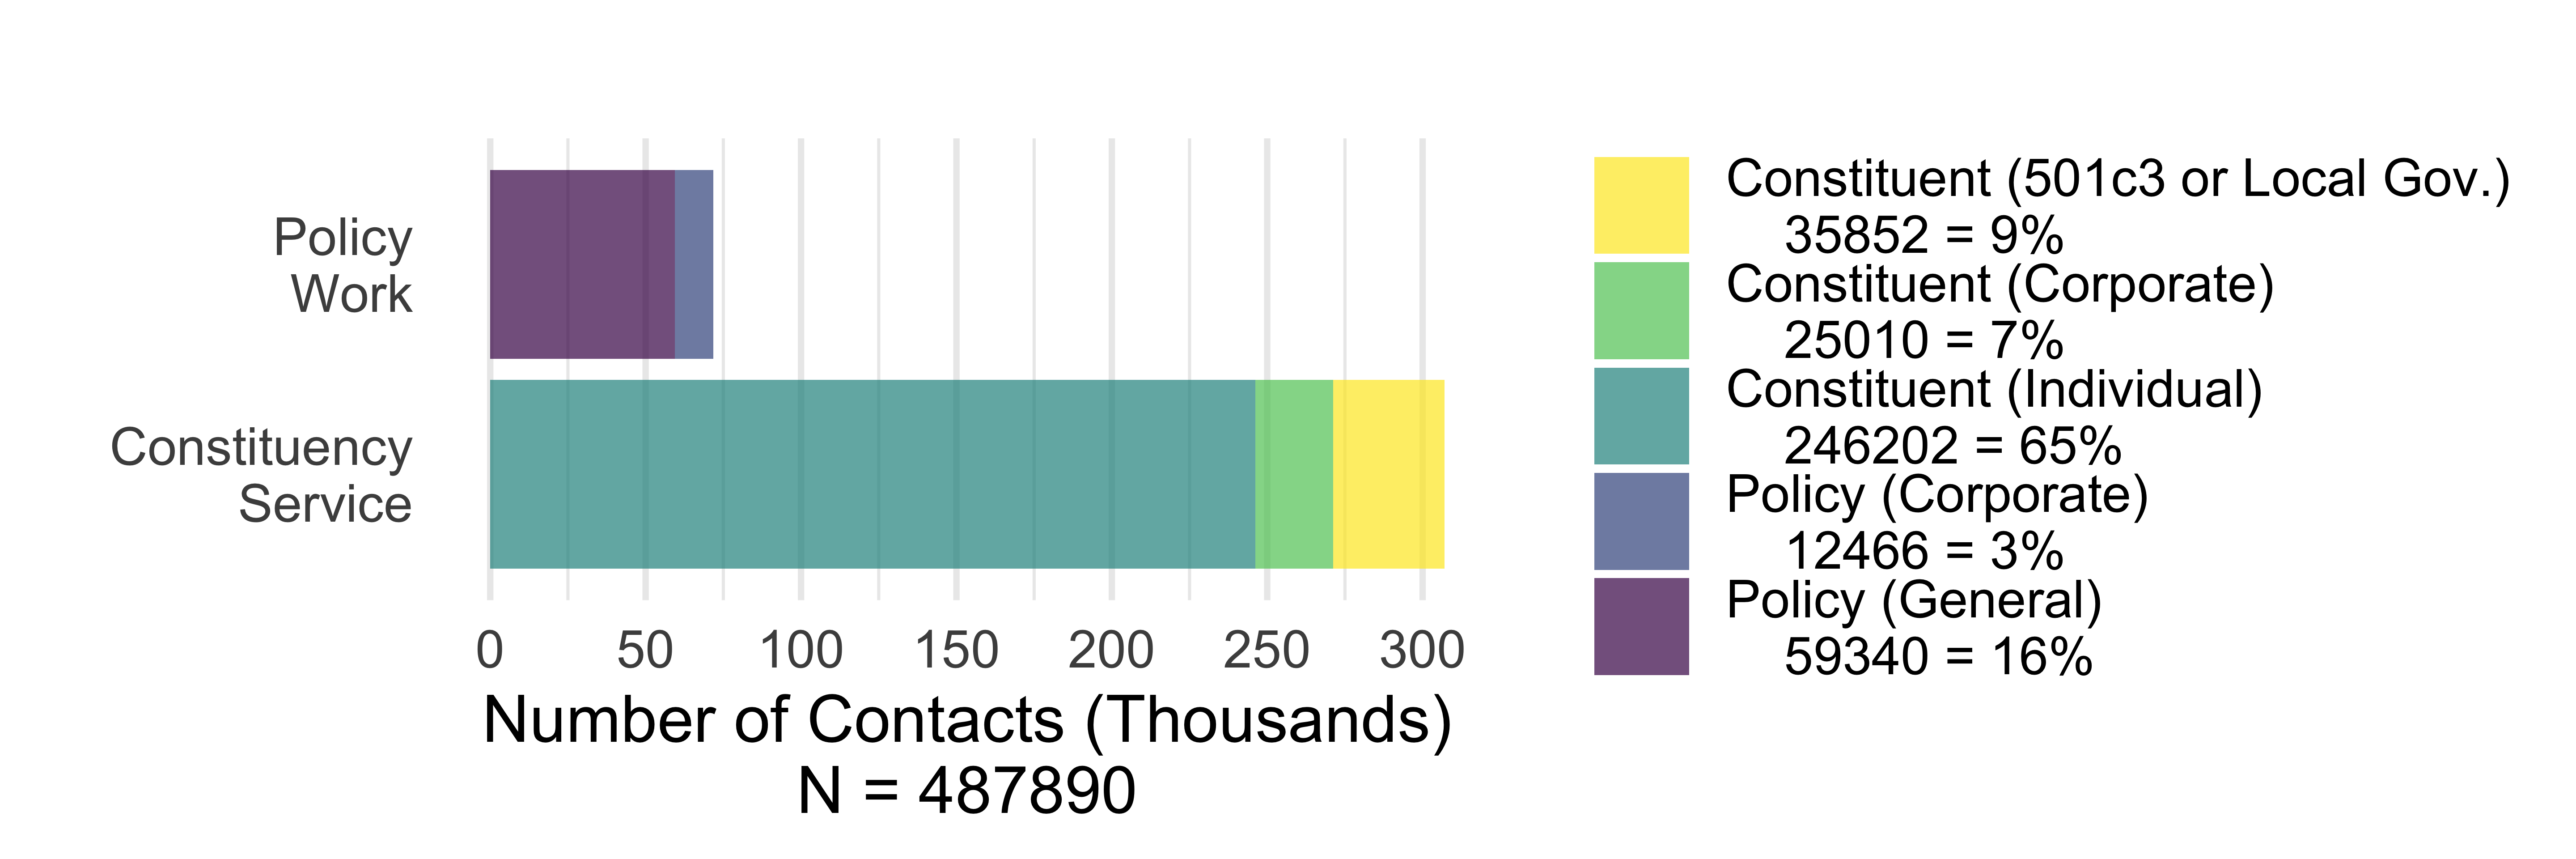
\includegraphics{../Figs/data_by_type-1}}
\end{figure}

The prevalence of constituency service requests is found across legislators regardless of their position in Congress or tenure in Washington.  To make these simple comparisons we will group together service for individuals, corporations, and non-profits into a ``constituency service" category, while allocating other policy contacts into a ``policy" category.  Using this more coarse classification, we find 82\% of contacts that chairs of committees make with federal agencies is focused on constituency service and 87.9\% of contacts from members of prestige committees is focused on constituent service.  Similarly, 89\% of the contacts legislators make in their first year are focused on constituency service and 87.5\% is focused on service in their sixth year. 

\subsubsection{Constituent Characteristics and the Provision of Constituency Service }

While legislators are focused on constituency service when they contact federal agencies, the characteristics of their districts helps inform the agencies that legislators contact.  We show now that population size and characteristics of constituents---the proportion who are veterans and the the proportion over 65---is correlated with how legislators make constituency service requests.  These correlations provide face-validations for our measures of legislative effort, but they also suggest that cross-sectional comparisons will conflate legislative effort with the characteristics of districts.  Given this potential conflation, our most stringent specifications below will include fixed effects for each legislator-agency pair, ensuring that we make within district comparisons.   

We should expect senators who represent larger states to make more service requests.  They have a larger number of constituents who might make requests of the senator.  And senators are allocated a larger budget to handle that increase in requests.  Figure \ref{f:stateSize} shows that this is the case: senators from larger states provide more constituency service on average.  This is true for senators from larger states, like John Cornyn (R-TX), Barbara Boxer (D-CA), and Pat Toomey (R-PA).  While there is an increase associated with population size, Figure \ref{f:stateSize} also shows that there is considerable across state variation in the amount of service senators provide.  

\begin{figure}
\centering
\caption{Senators from larger states do more constituent service.} \label{f:stateSize}
\scalebox{0.3}{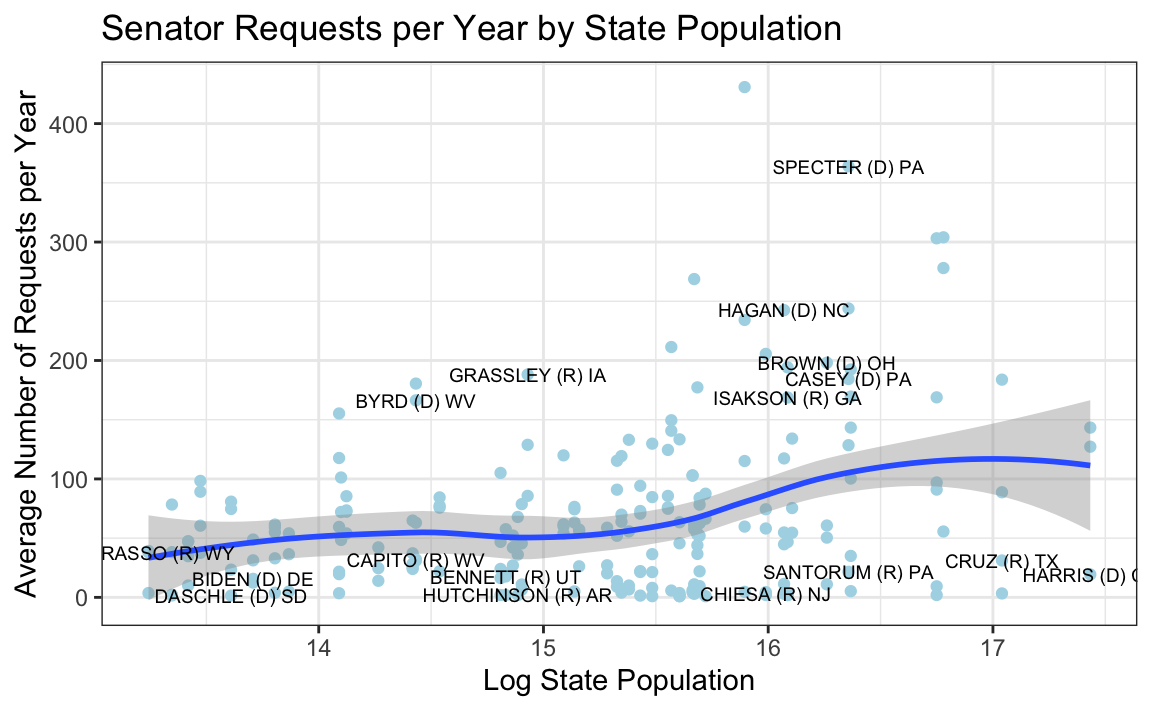
\includegraphics{../Figs/population-1}}
\end{figure}

The number of times legislators contact particular agencies is also correlated with the demographic composition of their districts.  To demonstrate the correlation between demographic characteristics and the rates legislators contact agencies, we focus on two example agencies: the Veterans Administration (VA) and the Social Security Administration (SSA). We measured the prevalence of two groups in the district: veterans---the residents who might plausibly need assistance navigating the VA---and residents who are over 65 years of age---and therefore satisfy the age eligibility for social security. We then ran a simple bivariate regression of the total number of contacts a legislator made of the agency on the proportion of constituents who are veterans or who are over 65.  

In both instances we find a correlation between district composition and the number of times legislators contact the agency.  For example, for the VA we find that 1 percentage point increase in the proportion of residents who are veterans is associated with an increase of about .84 constituency service requests to the agency. Similarly, a one percentage point increase in the proportion of residents over 65 is associated with an increase of an additional 0.03 requests made to the agency. Overall, this suggests legislators' efforts are correlated with the district's demographic composition.  


\section{Assessing The Effect of Changing Positions and Increased Experience in Washington on Constituency Service}\label{s:prestige} 

Using this data set of federal contacts, we now assess how legislators' changing position in Congress affects their provision of constituency service.  Our primary models will be a series of difference-in-differences regressions, which are similar to the specifications in \cite{BerryFowler2016}.  Our most stringent specification will examine changes that are within legislator and agency.  Specifically, we will estimate regressions of the form: 

\begin{eqnarray}
Y_{ijt} & = & \boldsymbol{\beta}^{'} \textbf{Committee Position}_{it}   + \sum_{s = 1}^{6} \eta_{s} \text{I}\left(\text{tenure}_{it} = s\right) + \gamma_{ij} +  \delta_{jt} +  m_{it} + p_{it} +  \epsilon_{ijt} \label{e:diff1}
\end{eqnarray}

Where $Y_{ijt}$ represents the number of requests legislator $i$ makes to agency $j$ in year $t$, so our analysis in this section takes place at the legislator-agency-year level.  $\gamma_{ij}$ is a fixed effect for the legislator-agency dyad.  This fixed effect accounts for individual characteristics of legislators, such as legislators who are more skillful at filling constituency service requests than other legislators.  Critically for our research design, this fixed effect also enables us to account for time-invariant constituent demand for constituency service with an agency, ensuring our results are not driven only by constituent demand.  It also accounts for characteristics such as the population of a state, demographic characteristics of its residents, and local industries that might be particularly likely to request help with specific agencies.  And it also ensures that we adjust for the different time periods agency data is available.  $\delta_{jt}$ is an agency-year fixed effect, takes into account agency-level common shocks across legislators in the provision of constituency service.    

Assuming that legislators' trends contacting agencies to provide constituency service follows parallel paths, $\boldsymbol{\beta}$ represents the average effect of changing prestige on a legislator's provision on constituency service.  We focus on three measures of a legislator's committee position: (1) whether they are a committee chair, (2) whether they are a ranking member of a committee, and (3) whether they are members of a prestige committee.  We focus on these four committee assignments because each represent different ways a legislators can acquire more power while in Washington.  As a legislator becomes a committee chair or ranking member, they have increased responsibilities when drafting and revising legislation and they have increased access to and control of committee resources to accomplish policy goals---in particular, the use of committee staff.  Similarly, legislators who join more prestigious committees are given the opportunity to shepherd national level policy through the legislative process.\footnote{We say that a House member is on a prestige committee if they are on Appropriations, Ways and Means, Rules, Budget, or Armed Services and if a senator is on Rules, Foreign Relations, Commerce, Budget, Armed Services, or Appropriations.} 

As \cite{BerryFowler2016} note, changes in legislators' committee assignments are often due to circumstances outside of the legislator's control, such as changing majority status, retirements on committee, or exclusion due to losses from a prior election \citep{GrimmerPowell2013}.  For the parallel trends assumptions to be violated, it would need to be the case that legislators differentially altered their rates of constituency service in anticipation of joining particular committees. To make this assumption more plausible we include a series of controls that capture time-varying characteristics of a legislator that might confound our inference about the effect of committee prestige. A particular concern is that legislators obtain new committee assignments when their party moves into or out of the majority or at the same time as the president party changes.  To address these concerns, we include an indicator for whether the legislator's party is the majority in year $t$, $m_{it}$ and if the member of Congress is from the same party as the president in year $t$, $p_{it}$.  Throughout, we cluster our standard errors at the legislator level.

In this same regression we also include indicators for legislators first six years in Congress,  $ \sum_{s = 1}^{6} \eta_{s} \text{tenure}_{it}$.  The effects of interest $\eta_{1}, \eta_{2}, \hdots, \eta_{6}$ describe how a legislator's provision of constituency service in a particular year differs from legislators who serve beyond 7 years.  We focus on the provision of constituency service over the first 6 years of a legislators tenure in Washington in order to assess how the provision of service from a legislator changes over their initial years in Washington, in order to capture the extent to which new legislators face start-up costs. This specification, however, is ill equipped to assess how electing a new representative affects the amount of constituency service a constituent receives.  To address this, in Section \ref{s:tenure_dist} we examine how electing a new representative affects the number of constituency service requests made on behalf of a district with a different difference-in-differences specification, at the district-year level.    

\section{The Effect of Increased Power on the Provision of Constituency Service}
Table \ref{t:prestige1} provides the coefficient estimates from Equation \ref{e:diff1}. We focus first on the estimated effect of increased committee prestige.  Table \ref{t:prestige1} shows that as legislators' acquire more prestige, their rates of constituency service increase. This is true in a cross-sectional comparison of legislators.  The first column of Table \ref{t:prestige1} excludes the legislator $\times$ agency  and year $\times$ agency fixed effects, but does include controls for majority status and being from the same party as the president.  Table 1 shows that committee chairs, ranking members, members of prestige committees, and members of the oversight committee provide substantially more constituency service than other legislators.  These differences, though, conflate legislators' overall ability with their position in Washington.  If legislators who are better at their jobs or who exert more effort are also selected for more prestigious committees, then the estimates from the first column of Table 1 confound legislators' overall ability with their institutional position.    


\begin{table}[hbt!]
\caption{Estimating the Effect of Increased Prestige and Tenure on Constituency Service Provision} \label{t:prestige1}

\begin{minipage}{\textwidth}
\begin{center}
\begin{tabular}{l*{4}{c}}
\toprule
                    &\multicolumn{1}{c}{(1)}&\multicolumn{1}{c}{(2)}&\multicolumn{1}{c}{(3)}&\multicolumn{1}{c}{(4)}\\
\midrule
Committee Chair     &       0.712&       0.206&       0.209&      0.0366\\
                    &     (0.152)&    (0.0951)&    (0.0951)&    (0.0136)\\
Ranking Member      &       0.852&       0.123&       0.136&      0.0250\\
                    &     (0.156)&    (0.0967)&    (0.0970)&    (0.0119)\\
Prestige Committee  &       0.470&      0.0790&      0.0746&      0.0210\\
                    &    (0.0665)&    (0.0508)&    (0.0519)&    (0.0103)\\
First Year          &      -0.255&      -0.139&      -0.144&     -0.0124\\
                    &    (0.0519)&    (0.0489)&    (0.0473)&   (0.00979)\\
Second Year         &     -0.0713&      0.0177&      0.0248&      0.0239\\
                    &    (0.0585)&    (0.0474)&    (0.0469)&   (0.00908)\\
Third Year          &     -0.0198&      0.0764&      0.0595&      0.0338\\
                    &    (0.0625)&    (0.0450)&    (0.0444)&   (0.00823)\\
Fourth Year         &     0.00126&      0.0707&      0.0522&      0.0260\\
                    &    (0.0664)&    (0.0455)&    (0.0431)&   (0.00806)\\
Fifth Year          &     -0.0515&      0.0280&      0.0266&      0.0164\\
                    &    (0.0611)&    (0.0377)&    (0.0367)&   (0.00701)\\
Sixth Year          &     -0.0156&      0.0504&      0.0744&    0.000378\\
                    &    (0.0728)&    (0.0536)&    (0.0516)&   (0.00762)\\
\midrule
Majority, President's Party&  \checkmark&  \checkmark&  \checkmark&  \checkmark\\
Legislator $\times$ Agency Fixed Effects&            &  \checkmark&  \checkmark&  \checkmark\\
Year $\times$ Agency Fixed Effects&            &  \checkmark&  \checkmark&  \checkmark\\
All Legislators     &  \checkmark&  \checkmark&            &  \checkmark\\
Serve At Least Second Term&            &            &  \checkmark&            \\
Dependent Variable  &       Count&       Count&       Count&Log(Count + 1)\\
Observations        &      412111&      412111&      388997&      412111\\
\bottomrule
\multicolumn{5}{l}{\footnotesize Robust standard errors in parentheses, clustered at legislator level}\\
\end{tabular}

\end{center}
\footnotetext{Column 1 shows the average differences across committee assignments and years in Congress.  Column 2 presents the difference-in-differences estimates. Column 3 subsets to legislators who serve at least 3 years in Congress. Column 4 takes the Log of the counts + 1 as the dependent variable.}
\end{minipage}
\end{table}

To address this confounding, the estimates from Column 2 of Table \ref{t:prestige1} provides the estimated effects from the difference-in-differences specification in Equation \ref{e:diff1}.  Across all four measures of committee prestige, we find that improved positions in the institution cause legislators to increase the amount of constituency service.  Consider first the effect of being a committee chair.  We estimate that becoming a committee chair causes an increase of 0.206 constituency service requests per agency (95-percent confidence interval [0.02, 0.39]).  Across all agencies, this represents an increase of approximately 13.6 additional constituency service requests or an increase that is about 20\% of the average number of contacts per agency in our data set. There is a smaller increase for individuals who become a ranking member and for those who join a Prestige Committee, though the increase is statistically significant for the prestige committee.  Becoming a ranking member of a committee causes an increase of 0.123 contacts per agency, while joining a prestige committee causes a 0.079 per agency increase in the number of constituency service contacts a member of Congress makes.

The findings in Table \ref{t:prestige1} are robust to alternative specifications and different formulations of the dependent variable.  For example, we might concerned that legislators with particularly high rates of constituency service are driving the results.  The fourth column shows that we obtain the same findings if we use $\log (Y_{ijt} + 1)$ in our difference-in-differences specification. Further, our results are not due to differential attrition.  The third column shows that we obtain nearly identical results if we restrict our analysis to legislators who serve beyond at least three years.      


\subsection{Minimal Changes in the Subject of Legislators' Requests}
As legislators obtain more prestigious committee assignments in Washington they increase the number of times they contact federal agencies.  While we have already shown that the vast majority of contact with federal agencies is focused on constituency service, it might be the case that the increased contacts are focused on issues not related to providing constituency service.  This could be particularly plausible when legislators acquire positions on committees with oversight over a particular federal agency.  Even legislators with prestigious committee assignments are largely contacting federal agencies to perform constituency service and that the increase in constituency service that occurs with increased prestige cannot be explained by only an increase policy focused requests.  Increased rates of contact does, in fact, reflect increased particularistic goods for the district.   


\begin{table}
\begin{center}
\begin{minipage}{\textwidth}
\caption{The Effect of Prestige and Tenure on the Proportion of Contacts Focused on Constituency Service} \label{t:contact_types}
\centering
\begin{tabular}{l*{2}{c}}
\toprule
                    &\multicolumn{1}{c}{(1)}&\multicolumn{1}{c}{(2)}\\
\midrule
Prestige            &      0.0220&     -0.0105\\
                    &   (0.00777)&    (0.0101)\\
Chair               &     -0.0744&     -0.0875\\
                    &    (0.0157)&    (0.0175)\\
Ranking Minority    &    0.000387&     -0.0346\\
                    &    (0.0138)&    (0.0142)\\
First Year          &      0.0428&      0.0223\\
                    &   (0.00918)&    (0.0115)\\
Second Year         &      0.0744&      0.0546\\
                    &   (0.00888)&    (0.0111)\\
Third Year          &      0.0400&      0.0235\\
                    &   (0.00888)&    (0.0107)\\
Fourth Year         &      0.0357&      0.0192\\
                    &   (0.00970)&    (0.0108)\\
Fifth Year          &     0.00801&    -0.00254\\
                    &   (0.00994)&    (0.0105)\\
Sixth Year          &      0.0533&      0.0431\\
                    &   (0.00933)&   (0.00940)\\
\midrule
Majority            &            &  \checkmark\\
Legislator Fixed Effects&            &  \checkmark\\
Year Fixed Effects  &            &  \checkmark\\
Observations        &        6442&        6442\\
\bottomrule
\multicolumn{3}{l}{\footnotesize Robust standard errors in parentheses, clustered at legislator level}\\
\end{tabular}

\footnotetext{This table shows how the proportion of contacts focused on constituency service changes as legislators acquire more power and experience in Washington.  Overall this demonstrates that the increased number of contacts with federal agencies from more experienced and prestigious legislators results in more constituency service.}
\end{minipage}
\end{center}
\end{table}

%%%%% Devin is the 77.2% Stat below correct?  This seems to contradict an earlier stat we provided. 
To describe what legislators contact federal agencies about, we use the hand classification codes from Section \ref{s:data} and code each of the contacts with federal agencies as either constituency service or policy focused.  Overall, 77.2\% of the average legislators' contacts with agencies are about constituency service.  The first column of Table \ref{t:contact_types} describes how the proportion of contacts that are constituency service differs over legislators' first six years in office and for legislators who have increased committee influence. This shows that a higher proportion of contacts from legislators are focused on constituency service in legislators initial years in office, but overall all legislators are allocating the vast majority of their contacts towards providing constituency service. 

Our research design is unable to identify the effect of increased tenure on the types of contacts legislators make, because to make the assessment it implicitly requires conditioning on a post-treatment variable: contacting federal agencies.  Nonetheless, a difference-in-differences regression can provide interesting descriptive evidence about how the content of legislators' contact with federal agencies changes as they gain more experience.  To that end, Column 2 uses a difference-in-differences regression to assess how tenure in Washington affects the proportion of contacts focused on constituency service. While there are significant changes in the proportion focused on constituency service, we still find that the vast majority of contacts are focused on constituency service.  This ensures that the additional contacts from increased tenure result in additional constituent service requests. 


\paragraph{Increased Power and Increased Constituency Service} In this Section we have shown that acquiring power in Washington causes legislators to increase their production of constituency service at home.  This increase occurs across all three measures of committee position that we examine, but is strongest for committee chairs. Further, we show that there are only small effects on the types of contacts legislators make, with even more powerful legislators focused primarily on constituency service.  Using a heterogeneous treatment effect model, we have shown that the increase in constituency service is consistent with both legislators having access to increased resources and a higher likelihood of success when contacting agencies. Rather than forgetting about the district and contracting Potomac Fever, it would appear that more power in policy making enables legislators to more effectively deliver particularistic goods to the district.  

\subsection{The Effect of Increased Experience in Washington on the Provision of Constituency Service}\label{s:tenure}

As legislators acquire more power in Washington, we find that they increase their provision of constituency service.  While this suggests that more powerful legislators are paying more attention to their constituents, it could still be the case that as legislators gain experience in Washington, they decrease their provision of constituency service.  To first test whether this is the case, we use the estimates in Table \ref{t:prestige1}, but now focus on the coefficients in legislators' first six years in office.  The counterfactual in mind here is how a particular legislator's provision of service changes over the first six year in office, where we include aspects of the office such as committee staff and protocols for constituency service.\footnote{Note, that interpreting these coefficients does require that we assume the effects are linearly separable.  But this is a particular strong case, because most legislators do not become chairs, ranking members, join prestige committees or the oversight committee in their first six years in Washington. } 


The first column of Table \ref{t:prestige1} shows that there are large descriptive differences: legislators in their first year make many fewer contacts than more experienced legislators, with first year legislators making approximately 0.255 fewer requests per agency than legislators in their seventh year or beyond.  This difference shrinks in the second year and then is largely gone.  But we have to exercise caution when interpreting the differences in Column 1, because they conflate the effect of increased experience in Washington with the different characteristics of legislators at different phases of their career.    


% To test this hypothesis, we use a similar empirical approach that we used in the previous section, but now focus on the first years of an individual's service in Washington.  Specifically, we estimate a difference-in-differences regression  of the form: 

% \begin{eqnarray}
% Y_{ijt} & = & \sum_{s=1}^{6} \beta_{s} \text{tenure}_{s[it]} + \gamma_{ij} +  \delta_{t}  + m_{it} + p_{it} +  \epsilon_{ijt} \label{e:diff2}
% \end{eqnarray} 

% where we include fixed effects for each legislator-agency pair ($\gamma_{ij}$), a time fixed effect ($\delta_{t}$), and indicators for a legislator's status in the majority ($m_{it}$) or in the president's party ($p_{it}$).  


%We are interested in both the size of these coefficients--which inform how legislators' provision of constituency service compares to legislators who have remained in office longer than 7 years---and comparisons across the coefficients---which describe how the provision of constituency service changes over the first 6 years in office.  Our comparisons across these first years do not depend on how many years we include in the analysis, because we will make the same basic comparisons over these initial years.  But the ``reference" category can lead to slightly different conclusions about the amount of service individuals provide compared to establish members.  In this section we focus on these first years because this is the time frame for many term limit proposals.  Further, this is the range where we have the best evidence for the year-to-year shifts in how legislators provide service.  The restriction in Equation \ref{e:diff2} is not consequential for the conclusions that we reach: we show in Appendix ZZ, the basic patterns that we uncover are consistent regardless of how many years we include in our analysis.  And as we show in Section YY, we find similar patterns when we examine what occurs after a new legislator takes office. 

%The first column of Table \ref{t:tenure1} is a cross-sectional regression that compares the provision of constituency service across legislators' first 6 years in Congress, while also including indicator's for a legislator's majority party status and whether they are members of the president's party.  This descriptive regression shows that new legislators provide substantially lower levels of constituency service than their colleagues in their second year of service in Washington: legislators in their first year make about 0.135 fewer constituency service requests per agency than legislators in their second year and 0.2 fewer requests than legislators in their third year.  Across all six years we find that newer legislators are, on average, making fewer contacts with federal agencies than their more experienced colleagues.  


% \begin{table}[hbt!]
% \caption{Estimating Effect of Tenure on Constituency Service Provision} \label{t:tenure1}
% \begin{minipage} {\textwidth}
% \begin{center}
% \begin{tabular}{l*{4}{c}}
\toprule
                    &\multicolumn{1}{c}{(1)}&\multicolumn{1}{c}{(2)}&\multicolumn{1}{c}{(3)}&\multicolumn{1}{c}{(4)}\\
\midrule
First Year          &      -0.478&      -0.179&      -0.183&     -0.0317\\
                    &    (0.0349)&    (0.0347)&    (0.0351)&   (0.00527)\\
Second Year         &      -0.344&     -0.0665&     -0.0630&   -0.000440\\
                    &    (0.0375)&    (0.0335)&    (0.0337)&   (0.00510)\\
Third Year          &      -0.274&    -0.00694&    -0.00697&     0.00662\\
                    &    (0.0376)&    (0.0328)&    (0.0328)&   (0.00482)\\
Fourth Year         &      -0.237&      0.0200&      0.0200&      0.0126\\
                    &    (0.0409)&    (0.0310)&    (0.0310)&   (0.00470)\\
Fifth Year          &      -0.238&    0.000539&    0.000506&   -0.000442\\
                    &    (0.0388)&    (0.0296)&    (0.0296)&   (0.00434)\\
Sixth Year          &      -0.220&      0.0204&      0.0204&     0.00242\\
                    &    (0.0401)&    (0.0278)&    (0.0278)&   (0.00414)\\
\midrule
Majority, President's Party&  \checkmark&  \checkmark&  \checkmark&  \checkmark\\
Legislator $\times$ Agency Fixed Effects&            &  \checkmark&  \checkmark&  \checkmark\\
Year Fixed Effects  &            &  \checkmark&  \checkmark&  \checkmark\\
All Legislators     &  \checkmark&  \checkmark&            &  \checkmark\\
Serve At Least Second Term&            &            &  \checkmark&            \\
Dependent Variable  &       Count&       Count&       Count&Log(Count + 1)\\
Observations        &      337610&      337610&      330215&      337610\\
\bottomrule
\multicolumn{5}{l}{\footnotesize Robust standard errors in parentheses, clustered at legislator x agency level}\\
\end{tabular}

% \end{center}
% \footnotetext{This table shows.  Model 1: no fixed effects.  Model 2: legislator x agency and year model 3: only those legislators who survive their first election. }
% \end{minipage}
% \end{table}


To address the differences in legislators at different career stages, the second column of Table \ref{t:prestige1} estimates the difference-in-differences specification in Equation \ref{e:diff1} and we now focus on the tenure coefficients.  This demonstrates that legislators provide less constituency service in their first year in office and as they acquire experience in Washington, the differences subside as legislators provide additional service.  Legislators in their first year in office provide 0.16 fewer constituency service requests per agency than legislators in their second year and 0.215 fewer requests than legislators in their third year---both differences are statistically significant at conventional levels.  The overall increase in number of constituency service requests from a legislator's first to third year is similar in size to the increase that comes from becoming a member of the oversight committee: resulting in about 14.6 more constituency service requests per-year.  Once legislators enter their fourth year, however, we see that there are no longer systematic changes in their rate of service provision.  We find small and statistically insignificant differences for legislators in their fourth through sixth years.  This demonstrates that as legislators acquire experience, they make more contacts with federal agencies.  

As with the analysis of committee prestige, the findings in Table \ref{t:prestige1} are robust to alternative specifications.  We might be concerned that the set of legislators who serve in their third year are different than the legislators who serve in the first years.  If this were the case, then our findings would be the result of both the experience and expertise that comes from more years in Washington and House members who win reelection, an indication that they are better able to perform the job than other legislators.  To address the potential different samples in each year, the third column of Table \ref{t:prestige1} assesses the changes in the number of contacts of federal agencies for legislators who serve in Congress for at least three years.  This reveals a very similar pattern: legislators initially providing less constituency service in their first two years, then more contacts subsequently.  And Column 4 in Table \ref{t:prestige1} shows that the results are robust to analyzing $\log(Y_{ijt} + 1)$, ensuring that our results are not because of outliers.  

\subsection{Assessing the Effect of a New Representative on Constituency Service Requests}\label{s:tenure_dist}

Using a within-legislator comparison, we have found that legislators make fewer contacts with federal agencies in their first year in office, but the number of contacts with agencies stabilizes after their third year.  In this section we examine a related, though distinct, question: how does the provision of constituency service to a district change after the election of a new representative?  Rather than examining changes in the number of contacts by making a within-legislator comparison, we are now going to make a within-district comparison.  This enables us to assess how electing a new legislator affects the total number of contacts with the federal government a district's representative makes.  In other words, this enables us to assess the costs or benefit of a new elected official.    


In order to make this comparison, we change the level of our analysis and focus now on the number of contacts made from the representative of a particular state or district $i$ in a year $t$, $Y_{it}$.  As in the prior sections, we will use a difference-in-differences approach to take into account the specific characteristics of districts and over time changes in how legislators provide constituency service.  Specifically, we estimate regressions of the form: 


\begin{eqnarray}
Y_{it} & = & \beta_{1}\text{New Member}_{it} + \sum_{s = 2}^{6} \beta_{s} \text{tenure}_{s[it]} + \gamma_{i} + \delta_{t} + \epsilon_{it} \label{e:district1} 
\end{eqnarray}

Where $\gamma_{i}$ is a district specific fixed effect that takes into account the particular demographic characteristics of the district, along with the levels of demand from district residents.  $\delta_{t}$ is a year fixed effect that takes into account common shocks.  Our key effect of interest $\beta_{1}$ is the effect of a district electing a new representative, for districts that do elect a new representative over the course of our study.  In order to understand how the effect of a new representative changes over time, we also estimate the district level differences for a legislators second ($\beta_{2}$) through sixth-year ($\beta_{6})$.\footnote{It is worth noting that this treatment is fundamentally different for a district then the treatment we examined before, which was at the legislator level.  In each election the district faces the choice of either allowing their incumbent to acquire another term of tenure in the chamber or replacing her with a new member.  This is different than the within legislator comparison, because legislators are only able to acquire more tenure or leave the chamber.}


The first column of Table \ref{t:district2} provides a simple difference-in-means for districts represented by a new member and then for legislators through their first six years in office.  In this descriptive comparison, districts represented by new legislators receive substantially fewer constituency service requests to federal agencies.  On average, districts with a new representative have 35.2 fewer constituency service requests made on their behalf.  The magnitude of this difference shrinks for districts represented by legislators in their second year (23.75 fewer constituency service requests) and then reaches a relatively stable number for districts represented by legislators in their third through sixth years, with some slight evidence that legislators make more contacts in election years---the even numbered years of tenure for the vast majority of legislators in our sample. 



\begin{table}[hbt!]
\caption{The Effect of New Members on Number of Requests at the District Level} \label{t:district2}
\begin{minipage}{\textwidth}
\begin{center}
\begin{tabular}{l*{4}{c}}
\toprule
                    &\multicolumn{1}{c}{(1)}&\multicolumn{1}{c}{(2)}&\multicolumn{1}{c}{(3)}&\multicolumn{1}{c}{(4)}\\
\midrule
New Legislator      &      -35.23&      -35.55&      -14.89&      -123.5\\
                    &     (4.445)&     (4.500)&     (2.627)&     (13.84)\\
Legislator 2nd Year &      -23.75&      -20.31&      -4.402&      -79.99\\
                    &     (4.464)&     (3.949)&     (2.662)&     (11.34)\\
Legislator 3rd Year &      -13.08&      -13.53&      -1.630&      -49.48\\
                    &     (4.886)&     (4.448)&     (2.586)&     (16.07)\\
Legislator 4th Year &      -12.43&      -9.077&       0.268&      -26.92\\
                    &     (5.216)&     (4.276)&     (2.736)&     (16.30)\\
Legislator 5th Year &      -14.92&      -11.58&      -3.810&      -31.58\\
                    &     (4.416)&     (3.591)&     (2.128)&     (13.11)\\
Legislator 6th Year &      -13.56&      -5.216&      -1.638&      -2.500\\
                    &     (5.104)&     (3.790)&     (2.239)&     (14.46)\\
\midrule
District Fixed Effects&            &  \checkmark&  \checkmark&  \checkmark\\
Year Fixed Effects  &            &  \checkmark&  \checkmark&  \checkmark\\
All Districts       &  \checkmark&  \checkmark&            &            \\
House Only          &            &            &  \checkmark&            \\
Senate Only         &            &            &            &  \checkmark\\
Observations        &        6578&        6578&        5338&        1240\\
\bottomrule
\multicolumn{5}{l}{\footnotesize Robust standard errors in parentheses, clustered at district level}\\
\end{tabular}

\end{center}
\footnotetext{This table shows how constituent service at the district level changes over time.  Model 1 is a cross sectional comparison excluding district and year fixed effects.  The second column is a district x year difference in differences model.  Column 3 focuses the diff-in-diff on legislators who survive their first election. }
\end{minipage}
\end{table}


To account for differences in district size, demographics, and demand for constituency service, the second column estimates the difference-in-differences from Equation \ref{e:district1}.  In this specification we see a large causal effect of a new member taking over: electing a new member causes a decrease of 35.6 constituency service requests (95-percent confidence interval [-44.42 , -26.78]).  This represents a sizable change in the number of service requests representatives make on behalf of their new constituents.  The effect of electing a new representative, however, dissipates quickly. Districts represented by a legislator in her second year of service receive 12.01 fewer constituency service requests---still a substantively important decrease in contact with federal agencies, but nonetheless not as drastic as the first year decrease.  After the second year the differences are smaller in magnitude.  This phenomenon---new legislators providing substantially fewer contacts with federal agencies---is found when we examine the House (Column 3) and the Senate (Column 4), separately.  In short, it is clear that new legislators make fewer contacts for their constituents than well-established elected officials.   


\paragraph{The Costs of Newly Elected Members} Taken together, our results demonstrate that new legislators experience substantial start-up costs when newly elected and that when a new legislator represents a district, they receive much less constituency service.  Legislators in their first year provide much less constituency service than they do in their second year and reach a stable level of service in their third years.  Further, when districts elect a new representative or senator, they experience a sharp decrease in the amount of constituency service requests made on their behalf.  Rather than experienced legislators forgetting about their districts, then, our evidence suggests that newly elected legislators struggle to provide the levels of service that experienced legislators deliver to their constituents.  
 


\section{The Limited Effects of Constituency Demand}\label{s:demand} 

An alternative explanation for our results is that the amount of constituency service legislators provide is largely driven by constituency demand.  We have attempted to limit the influence in demand when assessing how power and experience affects the provision of constituency service.  For example, our empirical strategy in Sections \ref{s:prestige} and \ref{s:tenure} account for static demand based on characteristics of the district.  For example, districts composed of veterans might see more requests for assistance with the Veterans' Administration, or districts with older residents might have greater demand with the social security administration.  Because our analyses take into account either legislator-agency or district fixed effects, we compare how the levels of constituency service change holding constant these characteristics of the district.  

Yet, we might expect that constituents' requests could be driven by a legislator's changing power in Washington or prestige.  Constituents could, for example, direct more of their requests to legislators who are more powerful or who have been in Congress for a longer period of time.  In this section, we present evidence that additional constituent requests to legislators is unable to explain our results, even though we have shown that there is a correlation between the demographics of a district and the number of requests legislators send to particular agencies.  We demonstrate the limited effects of constituency service using two distinct approaches.  Building off the theoretical discussion in Section \ref{s:theory}, we might worry that legislators' increasing prestige leads them to have higher name recognition, causing constituents to direct more constituency service requests to them.  We show, however, that as legislators acquire more institutional power in Washington it does not cause an increase in name recognition.  While more experienced legislators do have higher name recognition, increases in name recognition do not align with the increases in constituency service that legislators provide their constituents, making name recognition a poor explanation for the increased number of contacts legislators make on behalf of their constituents.   

If how constituents direct their requests for service explains our results, then we might expect there to be spillover across legislators.  When new members are elected, constituents could direct their service requests to more experienced legislators who are better known to the constituent seeking help.  We show that when a district is represented by a new legislator, other members of Congress and same-state senators do not have an increase in the amount of constituency service provided.  This suggests that constituents are not merely redirecting their service requests to more experienced legislators.  Rather, members of Congress' are able to both solicit and fulfill constituency service requests when they have adequate staff.  As their staff budget expands, they able to fulfill more requests.  

\subsection{The Limited Effects of Prestige and Tenure on Name Recognition}
To assess how changing prestige and tenure affects legislator's name recognition, we use the Cooperative Congressional Election Study (CCES) cumulative file.  This collects a set of survey responses from 2006-2018, providing a total of 452,755 total individual level responses.  All respondents were asked if they approve of their representative in the US House and both senators.  If the respondent provided an assessment of the elected official, we coded the respondent as recognizing the legislator's name.  If, however, the respondent selected the option that they had never heard of the representative, or were not sure, then we code them as not recognizing the legislator.  

Given our focus on how legislators alter their name recognition among constituents, we estimate the average name recognition for each legislator in each survey $Y_{it}$, or the proportion of respondents who provide an evaluation of the legislator.  We then use cross-sectional and difference-in-differences regressions to assess how legislators name recognition changes as they acquire more experience and as they increase their institutional prestige.  

\begin{table}[hbt!]
\caption{Limited Changes in Name Recognition} \label{t:namerec1}

\begin{minipage}{\textwidth}
\begin{center}
\begin{tabular}{l*{2}{c}}
\toprule
                    &\multicolumn{1}{c}{(1)}&\multicolumn{1}{c}{(2)}\\
\midrule
Second Year         &     -0.0385&     -0.0230\\
                    &   (0.00642)&   (0.00641)\\
Fourth Year         &     -0.0263&    0.000275\\
                    &   (0.00646)&   (0.00682)\\
Sixth Year          &     -0.0281&     -0.0112\\
                    &   (0.00676)&   (0.00634)\\
Eighth Year         &     -0.0132&     0.00132\\
                    &   (0.00663)&   (0.00674)\\
\midrule
Legislator Fixed Effects&            &  \checkmark\\
Year Fixed Effects  &            &  \checkmark\\
Observations        &        3667&        3667\\
\bottomrule
\multicolumn{3}{l}{\footnotesize Robust standard errors in parentheses, clustered at legislator level}\\
\end{tabular}

\end{center}
\end{minipage}
\end{table}


The first column of Table \ref{t:namerec1} shows average levels of name recognition of legislators' tenure in the House and Senate.  This demonstrates that legislators who are newer to Congress have lower-levels of name recognition. Further, we continue to see lower-levels of name recognition for legislators at the end of their second year, then for legislators serving in their 10th year and beyond.  Yet, both the persistence of this difference and the rate at which is it resolved suggest that name recognition is likely to have only a limited explanation for why legislators receive more requests after their first year.  This is because even second-year legislators---when the decrease in constituency service has already begun to be resolved---continue to have lower name recognition.   


The third column of Table \ref{t:namerec1} shows that, on average, legislators who hold more power in Washington do have higher name recognition back in the district.  Yet, using a difference-in-differences design to make within-legislator comparisons over their careers, we see that these differences disappear.  Column 4 shows that when legislators acquire more power in Washington, it has little effect on their name recognition with constituents.  And finally, columns 5 and 6, which includes both tenure controls and prestige, shows the same basic pattern: increasing prestige in Washington does little to affect name recognition back in the district.  


\subsection{No Evidence Constituents Redirect Requests Away from New Legislators Towards Incumbent Legislators}
In this section we engage in a more direct test of whether constituent demand explains variation in how legislators provide constituency service.  If constituents are merely redirecting their requests for constituent service in response to characteristics of legislators, then we should expect that the number of requests that incumbent legislators make will increase when there are new representatives in their state.  We would expect an increase if constituent demand explained our results because constituents would direct their service requests away from the new legislator and towards incumbent legislators.  If this spillover occurs, then the most natural target for the constituent requests would be one of the senators representing the constituent's state, but a different House member could also receive the request.    

To assess the whether constituents direct requests towards incumbent legislators when new members represent them, we examine how incumbent legislators' constituency service requests change in response to having new representatives in their state.  We measure the presence of new member in the state in two ways: either the proportion of House members and senators in the state who are new or an indicator for whether there is a new House member or senator in the state.  As in the previous section, we measure the number of constituency service requests that are made from a districts representative in a particular year.  Using this dependent variable, we then estimate a series of difference-in-differences regression where the treatment is the measure of new members in the state and we include district and time fixed effects.  Further, we restrict the regression to incumbent legislators only.    

Table \ref{t:spill1} presents the estimates of this regression.  The first two columns are estimated on all incumbent legislators and show that neither the proportion of new members nor the presence of a new member significantly affect the constituency service requests for other legislators. Columns 3 and 4 of Table \ref{t:spill1} reveal the same pattern when examining senators only.  Again, we see that the estimated effect of having a new legislator in the state and the proportion of new legislators is in the opposite direction than expected if spillover is occurring and does not approach statistical significance.  

    

\begin{table}[hbt!]
\caption{Little Evidence of Spillovers from New Legislators} \label{t:spill1}

\begin{minipage}{\textwidth}
\begin{center}
\begin{tabular}{l*{4}{c}}
\toprule
                    &\multicolumn{1}{c}{(1)}&\multicolumn{1}{c}{(2)}&\multicolumn{1}{c}{(3)}&\multicolumn{1}{c}{(4)}\\
\midrule
Proportion New Legislators&       5.143&            &      -1.494&            \\
                    &     (8.089)&            &     (20.06)&            \\
At Least One New Legislator&            &       1.625&            &       3.847\\
                    &            &     (2.031)&            &     (4.812)\\
\midrule
District Fixed Effects&  \checkmark&  \checkmark&  \checkmark&  \checkmark\\
Year Fixed Effects  &  \checkmark&  \checkmark&  \checkmark&  \checkmark\\
Senators Only       &            &            &  \checkmark&  \checkmark\\
Observations        &        6080&        6080&        1182&        1182\\
\bottomrule
\multicolumn{5}{l}{\footnotesize Robust standard errors in parentheses, clustered at district level}\\
\end{tabular}

\end{center}
\end{minipage}
\end{table}


\section{Conclusion} \label{s:conclude}

Using a new data set on constituency service requests made to federal agencies, we show that legislators increase their effort as they gain more power.  Even as legislators gain power the vast majority of requests legislators make is focused on constituency service.  And using a heterogeneous effect model, we have shown that the increase in requests made because of prestige are consistent with both an increase in resources and an increase in the likelihood of legislators success. Further, we show that legislators make fewer service requests at the start of their career and that new legislators make substantially fewer service requests than their more experienced colleagues,  

Our results are broadly consistent with the predictions about the provision of constituency service from multi-task selection models, such as \cite{AshworthBuenodeMesquita2006}.  Constituent service provides an incumbency advantage in these models because it provides legislators the opportunity to demonstrate their ability to constituents.  Our results show that legislators take advantage of this opportunity, particularly as they become more powerful.  Further, our results show that legislators will have an advantage in providing service over new representatives.  This provides an advantage because any switch in representation will necessarily imply a decline in particularistic services to the district. 

Our results also flip some of the concerns of term limit advocates on their head.  While a number of term limit advocates argue that elected officials will lose focus on their district, we show that the more experienced legislators provide more attention to their district.  There does not appear to be widespread outbreaks of Potomac Fever.  Rather, it appears that reelection oriented legislators are focused on providing service to the district to keep their place in Washington.   


\bibliography{congress2019}

%\newpage
%\listoftodos[Notes]

\clearpage
\appendix
\setcounter{table}{0}
\renewcommand{\thetable}{A\arabic{table}}

\section*{Appendix}

%%% Ellie: I manually changed the input code here so that the entire table would fit here.  
\input{../tables/FOIA_response.tex}


\section{Contact Codebook} \label{a:codebook}
\singlespacing
%%% Note: From Ellie.  I deleted everything here that we're not using in this paper.  

We provide the following codebook to a team of hand-coders to code the content of Congressional contact with legislative agencies and for extracting information about the legislator. The codebook provides a series of steps to move from raw correspondence logs to data formatted for the analysis conducted here.  

\subsection{Congressional Correspondence Log Coding Guidelines}

The first step is to identify the columns that contain the member of Congress (or Committee), the date that the member initiated correspondence, and the column that best describes the subject. These should be named FROM, DATE, and SUBJECT. 

Our aim is to classify the subject of correspondence between members of Congress and government agencies. This may be done using keywords (potential keywords in italics below), but may also require googling subject lines (e.g. what does this acronym mean in this context!?) and inferring why the request is being made. This may require identifying a member's relevant policy positions. For example, if the subject is "mining regulations" or "open internet," a member's voting history on related bills or donations from the industry may help us infer if the letter was policy work on behalf of the industry (type 4) or not (type 5). Limiting your search to a date range around the letter letter date may yield relevant public statements. If you have questions, find something interesting, or, in your efforts to classify a confusing correspondence, you discover information like a related public statement, note it in the NOTES column. In some cases, columns other than the SUBJECT may offer helpful information. This may be difficult at first, but will get easier. \\

The outcome is a spreadsheet with the first columns being FROM, DATE, SUBJECT, TYPE, CERTAINTY, ALT\_TYPE.\\

At the end of this codebook there are two tools:
\begin{tight_itemize}
\item[1)] An example for how to auto-apply these codes in R. 
\item[2)] A list of specific coding decisions for cases that required discussion among our team--please read through and add to this list as you encounter difficult cases. 
\end{tight_itemize}

Below are 5 potential codes for the TYPE and 3 potential codes for your level of CERTAINTY that it is this type. If you less than Very Certain (i.e. if only Fairly Certain, or Toss Up), also record your second best guess as ALT\_TYPE, otherwise leave this column blank. Only leave NOTES if you think it would be helpful for the team to revisit the entry.

\subsubsection{TYPE}

1 = Personal Service\\

\hfill\begin{minipage}{\dimexpr\textwidth-2cm}
Definition: Individual, non-commercial constituent service.\\
Examples: Help with a government form, passport, visa, back pay, military honor, enlistment, criminal case, request for personal information (e.g. one’s FBI file), disability application, worker compensation, personal complaint, discrimination case, job application, health insurance, financial services complaints, etc.\\
\end{minipage}

2 = Commercial Service - Transactional \\

\hfill\begin{minipage}{\dimexpr\textwidth-2cm}
Definition: Anything related to a specific individual case by a business (including business owners like farmers and consultants).\\ 
General Examples: Help with a grant application, payment, loan or contract (buying anything from or selling anything to a government agency). Help with an individual case of tax assessment, fine, or regulatory enforcement action. Help with public relations on behalf of a business.\\
Specific Examples: allocation of radio spectrum, case against a company, tax dispute, contract for purchase of military surplus, crop insurance distribution, debt settlement, foreclosure assistance, a fine for a law violation, etc. \\
\end{minipage}

3 = Government and Nonprofit Service - Transactional\\

\hfill\begin{minipage}{\dimexpr\textwidth-2cm}
Definition: Same as for (2-Commercial Service), but for municipal or state governments (including cities, counties, etc.) or non-business-oriented non-profit organizations (i.e. NOT ones that represents an industry or trade association) \\
\end{minipage}

4 = Commercial Service - Policy \\

\hfill\begin{minipage}{\dimexpr\textwidth-2cm}
Definition: Anything applying to a class of commercial activity or businesses (e.g. shipping, airlines, agriculture). This could include legislation, bills, acts, appropriations, authorizations, etc.  \\
General Examples: Authorization of or appropriation to a government program that is targeted towards a particular industry or industries. Regulation of an industry or commercial practice or competition.\\
Specific Examples: Milk prices, insurance or loan eligibility criteria, purchasing policies, crop insurance rates, pollution criteria, classification of products for trade or taxation, conservation appropriation, worker visa types, restrictions, or caps, etc.\\
\end{minipage}
 
5 = Policy Work - NOT in the service of any individual, business, specific industry.\\

\hfill\begin{minipage}{\dimexpr\textwidth-2cm}
Examples of Policy Work: 
 \begin{tight_itemize} 
  \item Lawmaking 
\item Request for policy-relevant information. This includes prospective legislation, legislation under consideration, or already implemented legislation that requires oversight.  
\item Oversight
\item Committee requesting a report or testimony at a hearing
\item  Requesting clarity on an agency rule
\item Lobbying administrative policy
\item Agency rulemaking with non-commercial implications (comments on agency rulemaking may often be (3)) 
\item Political work
\item Meeting with organized constituent groups (e.g. workers, people with disabilities, environmentalists) about policy (meetings with industry groups generally fall under (4)).
\item Media requests
 \end{tight_itemize} 
\end{minipage}
\bigskip


6 = Other \\

\hfill\begin{minipage}{\dimexpr\textwidth-2cm}
	Suggest a new category in the NOTES column, only if it cannot be fit under 1-4. For example, requesting dirt on one's political opponents could be called "partisan" as it is none of the above. Other specific types: thank you (for thank you notes with no other information), congratulations (for congratulatory correspondence on appointments or retirements with no other information), family member (for correspondence on behalf of a family member) \\
\end{minipage}

0  = Really no idea, no guesses, completely unclear \\
 

\subsubsection{CERTAINTY (regarding TYPE)} 
\begin{tight_itemize}
 \item[] 1 = Very Certain ($>$95\% sure).
\item[] 2 = Fairly Certain (between 95\% and 50\% sure).
\item[] 3 = Toss Up ($<$50\% sure).
\end{tight_itemize}

 
\bigskip
\textbf{Automated Coding Instructions:}
If you become confident that all entries containing a certain word or phrase are all one TYPE, we can save time by automatically applying this to all entries. This can be done in two ways:
\begin{tight_itemize}
\item[1)] If you are comfortable R, write a script, [agency].R that applies your rules. See example below.
\item[2)] If not, write classification rules in some standard intuitive way in the github issue for that agency. (For example, If "contract" in SUBJECT, TYPE = 2, CERTAINTY = 1.) Then ignore all future entries that meet your criteria (we will automatically apply your codes later).
\end{tight_itemize}

\newpage
\textbf{Automated Coding Example from {\tt USDA\_RD.R}:}

\hfill\begin{minipage}{\dimexpr\textwidth-2cm}
\begin{verbatim}
options(stringsAsFactors = FALSE)
library(tidyverse)
library(magrittr)
library(googledrive)
gs_ls() # log in to google drive
data <- gs_title("USDA_RD") %>% gs_read()   # get data from google drive
unique(data$SUBJECT) # view unique SUBJECT strings
data %<>% mutate(TYPE =
                      Ifelse (SUBJECT %in% c(
                        # i.e. if SUBJECT is exactly one of these strings:
                        "Payment Assistance",
                        "Delinquency ",
                        "Insurance ", 
                        "General Servicing",
                        "Foreclosure",
                        "Debt Settlement",
                        "Escrow  ",
                        "Recapture Receivable Account",
                        "Payoff "), 
                        2, TYPE)) # then make it TYPE 2
# Or, for imperfect matches (notice how some words above had random spaces 
# added), use "regular expression" matching. For example, with the 
# grepl() function:
?regex
?grepl
                    
data %<>% mutate(TYPE =
                      ifelse (grepl(
                       # i.e. if SUBJECT contains:
				 # (& means "AND",  | means "OR")
                        	"Payment|
Delinquency|
Insurance|
Servicing|
Foreclosure|
Debt Settlement|
Escrow|
Recapture Receivable Account|
Payoff", 
                        SUBJECT), 
                        2, TYPE))  # then make it TYPE 2, otherwise keep TYPE
# Notice how the odd spaces are no longer needed to return a match
# Also notice how "Payment Assistance" is now matched with just "Payment"
cbind(data$SUBJECT, data$TYPE) # view results
\end{verbatim}
\end{minipage}

\end{document}






 